%; whizzy paragraph -pdf xpdf -latex ./whizzypdfptex.sh
%; whizzy-paragraph "^\\\\begin{frame}\\|\\\\emtext"
% latex beamer presentation.
% platex, latex-beamer でコンパイルすることを想定。 

%     Tokyo Debian Meeting resources
%     Copyright (C) 2012 Junichi Uekawa

%     This program is free software; you can redistribute it and/or modify
%     it under the terms of the GNU General Public License as published by
%     the Free Software Foundation; either version 2 of the License, or
%     (at your option) any later version.

%     This program is distributed in the hope that it will be useful,
%     but WITHOUT ANY WARRANTY; without even the implied warreanty of
%     MERCHANTABILITY or FITNESS FOR A PARTICULAR PURPOSE.  See the
%     GNU General Public License for more details.

%     You should have received a copy of the GNU General Public License
%     along with this program; if not, write to the Free Software
%     Foundation, Inc., 51 Franklin St, Fifth Floor, Boston, MA  02110-1301 USA

\documentclass[cjk,dvipdfmx,12pt]{beamer}
\usetheme{Tokyo}
\usepackage{monthlypresentation}

%  preview (shell-command (concat "evince " (replace-regexp-in-string "tex$" "pdf"(buffer-file-name)) "&")) 
%  presentation (shell-command (concat "xpdf -fullscreen " (replace-regexp-in-string "tex$" "pdf"(buffer-file-name)) "&"))
%  presentation (shell-command (concat "evince " (replace-regexp-in-string "tex$" "pdf"(buffer-file-name)) "&"))

%http://www.naney.org/diki/dk/hyperref.html
%日本語EUC系環境の時
\AtBeginDvi{\special{pdf:tounicode EUC-UCS2}}
%シフトJIS系環境の時
%\AtBeginDvi{\special{pdf:tounicode 90ms-RKSJ-UCS2}}

\title{東京エリアDebian勉強会}
\subtitle{第95回 2012年12月度}
\author{上川純一\\dancer@debian.org}
\date{2012年12月15日}
\logo{\includegraphics[width=8cm]{image200607/openlogo-light.eps}}

\begin{document}

\frame{\titlepage{}}

\begin{frame}{設営準備にご協力ください。}
会場設営よろしくおねがいします。
\end{frame}

\begin{frame}{Agenda}
\begin{minipage}[t]{0.45\hsize}
  \begin{itemize}
  \item 注意事項
	\begin{itemize}
	 \item 飲食禁止
	 \item 宗教禁止
	 \item 営利活動禁止
	\end{itemize}
   \item 最近あったDebian関連のイベント報告
	\begin{itemize}
        \item 第94回 東京エリアDebian勉強会
	\end{itemize}
   \item 事前課題紹介
 \end{itemize}
\end{minipage} 
\begin{minipage}[t]{0.45\hsize}
 \begin{itemize}
  \item im-config 
  \item 著作権法改正
  \item 2012年のDebian勉強会を振り返る
 \end{itemize}
\end{minipage}
\end{frame}

\emtext{事前課題}
{\footnotesize
 %; whizzy-master ../debianmeetingresume201212.tex
% 以上の設定をしているため、このファイルで M-x whizzytex すると、
% whizzytexが利用できます

\begin{prework}{ 吉野(yy\_y\_ja\_jp) }

\preworksection{DFSGにおいての自由について論じてください。}

 自由を守るための制限である。

\preworksection{Debianに関して、2012年をふりかえって2013年やっておきたいことを論じてください。}

 Bug squashing,DDTPなどでの翻訳
\end{prework}

\begin{prework}{ seiji-n }
\preworksection{DFSGにおいての自由について論じてください。}

5.すべての個人、団体の平等

6.ライセンスは、すべての個人や団体を差別してはなりません。

DFSGの上記各条項に関して、テロリスト等反社会団体や犯罪者、犯罪集団による
反社会的活動、犯罪行為への利用に対して、差別ではなくと区別はしており、
(規制はできないながらも)決して全面的に承認している訳ではないという
意志表明的な事をすべきではないか。なぜしないのか。その上での自由では
ないかと考えています。


目標分野の平等

\preworksection{Debianに関して、2012年をふりかえって2013年やっておきたいことを論じてください。}

恐縮ですが2012年はDebianに関して何もしていません。これから学んで行きたいと思います。

\end{prework}

\begin{prework}{ dictoss(杉本 典充) }

\preworksection{DFSGにおいての自由について論じてください。}

9番目の「ライセンスは他のソフトウェアを侵害しない」とある。LGPLライセンスはGFSG互換ライセンスだが実行時は他のソフトウェアの自由を侵害してる場合がありそうな気がするがどうなんだろうか。


\preworksection{Debianに関して、2012年をふりかえって2013年やっておきたいことを論じてください。}

今年はarmelアーキテクチャのdebianを初めて自分でインストールしてみた。先人達の知恵があるため割とすんなり入ってしまってdebianはすごいと思った。来年はmips系のハードを探してdebianを入れて色々試してみたいと思います。
\end{prework}

\begin{prework}{ キタハラ }
\preworksection{DFSGにおいての自由について論じてください。}

 論じる程の知能はないので、替わりに感想を。
他のライセンス等に比べ、間口が広く、現実的で、制限が少なく、
開発者のみならず利用者にも心地のよい自由であると思う。

\preworksection{Debianに関して、2012年をふりかえって2013年やっておきたいことを論じてください。}
 私事ですが、異動で使えなくなったDebian社内サーバの代わりを何とかしたいですね。
\end{prework}

\begin{prework}{ 石井一夫 }

\preworksection{DFSGにおいての自由について論じてください。}

よくわかりませんが、ソースコードの公開とその運用の自由は維持してほしいです。

\preworksection{Debianに関して、2012年をふりかえって2013年やっておきたいことを論じてください。}

ビッグデータ関係が、主戦場になっています。ZFSの適用、セキュリティの強化の面から、kfreeBSDに注目しています。2013年は、ビッグデータとkfreeBSDでなにか貢献ができればと考えています。
\end{prework}

\begin{prework}{ akikazu.sudou }

\preworksection{DFSGにおいての自由について論じてください。}

よく知らないけれど、DFSGのおかげで今のdebianが使えるのなら、ありがたいものだと思います。

\preworksection{Debianに関して、2012年をふりかえって2013年やっておきたいことを論じてください。}
debianホストの仮想環境をいじってみたいです。

\end{prework}

\begin{prework}{ なかおけいすけ }
\preworksection{DFSGにおいての自由について論じてください。}

 Debianは、Debian社会契約により、Debianシステムとその構成要素が100\%フ
 リーソフトウェアでなければならないと規定しています。その著作物が「フリー」
 であると判断するための基準がDFSGです。すなわち、Debianに含まれるソフト
 ウェアは、再配布する自由、個人や団体、目的によらず使用する自由、および
 改変する自由をユーザーに与えるものでなければなりません。

 特に目的如何に問わずソフトウェアを使用する自由と、ソースコードを入手し、
 かつ改変する自由は、開発元がサポートをやめたとしても、(やろうと思えば)
 ユーザが自分たちでなんとかできるということです。これは長期間システムを
 維持することを求められる現場において非常に強力な武器になります。

\end{prework}

\begin{prework}{ 野島 貴英 }

\preworksection{DFSGにおいての自由について論じてください。}
 debianを主に使ってると、なんかもう空気のような当たり前の存在に感じてし
 まうDFSGです。ここでうたわれている自由は、エンジニアライフにとって最低
 限不可欠な自由だと個人的には思ってます。ただ、自分の知見が足らない為か、
 実はDFSGでうたわれている自由がどんな事を犠牲にして、どんな努力でささえ
 られているのかがあまりよく解っておらず...このあたり誰か教えてーっ。

\preworksection{Debianに関して、2012年をふりかえって2013年やっておきたいことを論じてください。}

 2012年は、おかげさまで、ちょっとはアウトプットできた?2013年はさらにアウトプット(ハック等)に励みまうす。
\end{prework}

\begin{prework}{ koedoyoshida }

\preworksection{DFSGにおいての自由について論じてください。}

ソフトウェア開発者のための自由ですね。
ある意味極北のディストリビューションであり、Debianの最大の特徴だとおもいます。
Ubuntuとの最大の違いといっても良いのではないでしょうか。

\preworksection{Debianに関して、2012年をふりかえって2013年やっておきたいことを論じてください。}

DebianJP参加。
\end{prework}

\begin{prework}{ yamamoto }
\preworksection{DFSGにおいての自由について論じてください。}

DFSG は、ソフトウェアの自由を確保するためには、なかなかよくできたガイド
 ラインだと思います。これにいくつかの事項を加えて OSD としたのも納得でき
 ます。また、完全にボランティアベースである Debian には、 ``フリーソフト
 ウェアコミュニティとの「社会契約」'' と共に、Debian が理想とするあり方を明示し、これらに賛同する者たちを集めるには必要なものと考えます。また DFSG フリーを保証することで、派生ディストリビューションなどの二次配布物の作成を容易にしたとも言えるでしょう。

ただし、例えば理想をひたすら追い求める RMS とかとは違い、Debian は DFSG
 フリーなソフトウェアだけでは成り立たない現実も理解していて、``フリーソ
 フトウェアコミュニティとの「社会契約」''の第一項では``Debian は 100\%
 フリーソフトウェアであり続けます'' とありますが、第五項の ``私たちのフ
 リーソフトウェア基準に合致しない著作物について'' において、non-free や
 contrib リポジトリの作成を謳っています。もちろん第一項により、これらは
 正式な Debian のパッケージとは言えませんが、BTS などでその配布物に関す
 る問題発生などを監視したりすることなどにより、利用をサポートしたり配布
 したりしています。 

これらの「理想」と「現実」の折り合いをつける感覚が、私はとても気に入っています。

\preworksection{Debianに関して、2012年をふりかえって2013年やっておきたいことを論じてください。}

特に無いかな?
\end{prework}

\begin{prework}{ 野首 }
\preworksection{DFSGにおいての自由について論じてください。}
 DFSGは「開発者」「配布者」「利用者」3者がバランスよく自由を享受できるようにしたものだと考えています。それぞれがかなりギリギリのラインをとっているように感じているので、今後変更されることはおそらくないように思います。

\preworksection{Debianに関して、2012年をふりかえって2013年やっておきたいことを論じてください。}
 全てのパッケージをきちんとformat 3に対応させたいところです。あとはvcs-buildpackageの利用促進と外部への公開も進めたいところ。

\end{prework}

\begin{prework}{ osamu@debian.org }

\preworksection{DFSGにおいての自由について論じてください。}
 DFSGの定義に賛成なんですが、FSFとのギャップの現実的解決策は、大事なことを忘れずいい意味での「寛容」なスタンスが双方必要かな?

\preworksection{Debianに関して、2012年をふりかえって2013年やっておきたいことを論じてください。}
日本語入力のim-configへの移行と改善ができたのが2012年、gnome-shellの最新版(>3.6)への対応が2013年の課題。

\end{prework}

\begin{prework}{ まえだこうへい }

\preworksection{DFSGにおいての自由について論じてください。}
 「すべての個人、団体の平等」「目標分野の平等」があるおかげで、利用目的、使い方関わらず、自由に使える恩恵を享受しています。一方、フリーソフトウェア、もしくはOSSではなく、単にソースコードが公開されているということで満足している人もいると感じます。そういう人がDebianやその派生物を利用するのもまた自由なので、DFSGに賛同する人が増えるよう活動を続けていく必要があるのかなと思います。

\preworksection{Debianに関して、2012年をふりかえって2013年やっておきたいことを論じてください。}
 今年は特に活動できなかったので、時間を作れるようにすることが第一。メンテナンスできてないパッケージや、ITPしたままになっているのとか、やる事は多いです。あとは来年も大統一Debian勉強会やりたいですね。
\end{prework}


}

\emtext{im-config}
\emtext{日本においてのDFSGの求める自由と2012年改正著作権法}

\begin{frame}{ソフトウェアの自由関連の2012年の流れと大きなイベント}
 \begin{itemize}
  \item 著作権法改正
  \item iOSデバイスなどのマーケットからしかソフトウェアがインストールで
	きないハードウェアの普及
 \end{itemize}
\end{frame}

\begin{frame}{2012年改正著作権法}
\begin{enumerate}
 \item  いわゆる「写り込み」(付随対象著作物の利用)等に係る規定の整備
 \item  国立国会図書館による図書館資料の自動公衆送信等に係る規定の整備
 \item  公文書等の管理に関する法律等に基づく利用に係る規定の整備
 \item  著作権等の技術的保護手段に係る規定の整備
 \item  違法ダウンロードの刑事罰化に係る規定の整備 
\end{enumerate}
 「平成24年通常国会 著作権法改正について」
\url{http://www.bunka.go.jp/chosakuken/24_houkaisei.html}
\end{frame}

\emtext{2012年のDebian勉強会}

\begin{frame}{2012年のテーマ}
  \begin{tabular}{|l|c|p{17em}|}
 \hline
 & 人数 & 内容\\
 \hline
   2012年1月 & 8 & Debian勉強会予約システム,VPS, twitter, 
	   月刊デブヘルパー, 2012年計画\\
   2012年2月 & 4? & KDE開発, 月刊デブヘルパー, cmake,  第0回福岡勉強会\\
   2012年3月 & ? & OSC \\
   2012年4月 & 13 & node.js, androidでDebian, 月刊デブヘルパー\\
   2012年5月 & 14 & coffeescript,python\\
   2012年6月 & ? & 大統一Debian勉強会 \\
   2012年7月 & 8? & MacBook Air 2011\\
   2012年8月 & 6? & Debconf 2012,月刊デブヘルパー,C++11 \\
   2012年9月 & 12 & OSC Tokyo Fall\\
   2012年10月 & 10 & Haskell, レゴ, xf86-input-mtrack\\
   2012年11月 & 14 & bluetooth tethering, linux perf, systemd\\
   2012年12月 & ? & 忘年会 \\
 \hline
\end{tabular}
\end{frame}

\begin{frame}{出席数推移}
\includegraphics[width=0.7\hsize,angle=270]{image201212/memberanalysis/attend.eps}
\end{frame}

\begin{frame}{事前課題推移}
\includegraphics[width=0.7\hsize,angle=270]{image201212/memberanalysis/prework.eps}
\end{frame}

\begin{frame}{2012年のテーマ}

何?

\end{frame}


\section{今後のイベント}
\emtext{今後のイベント}
\begin{frame}{今後のイベント}
\begin{itemize}
 \item 2013年1月 Debian 勉強会
\end{itemize}
\end{frame}

\section{今日の宴会場所}
\emtext{今日の宴会場所}
\begin{frame}{今日の宴会場所}
 荻窪「はなの舞」にて。
\end{frame}

\end{document}

;;; Local Variables: ***
;;; outline-regexp: "\\([ 	]*\\\\\\(documentstyle\\|documentclass\\|emtext\\|section\\|begin{frame}\\)\\*?[ 	]*[[{]\\|[]+\\)" ***
;;; End: ***
